\documentclass{standalone}
\usepackage{tikz}
\usetikzlibrary{patterns}
\usetikzlibrary{positioning}
\usetikzlibrary{patterns, positioning}
\usetikzlibrary{shapes.misc}
\usepackage[outline]{contour}
\contourlength{1.5pt} 
\usetikzlibrary{calc}
        \usepackage{relsize}
        \tikzset{fontscale/.style = {font=\relsize{#1}}}

\begin{document}
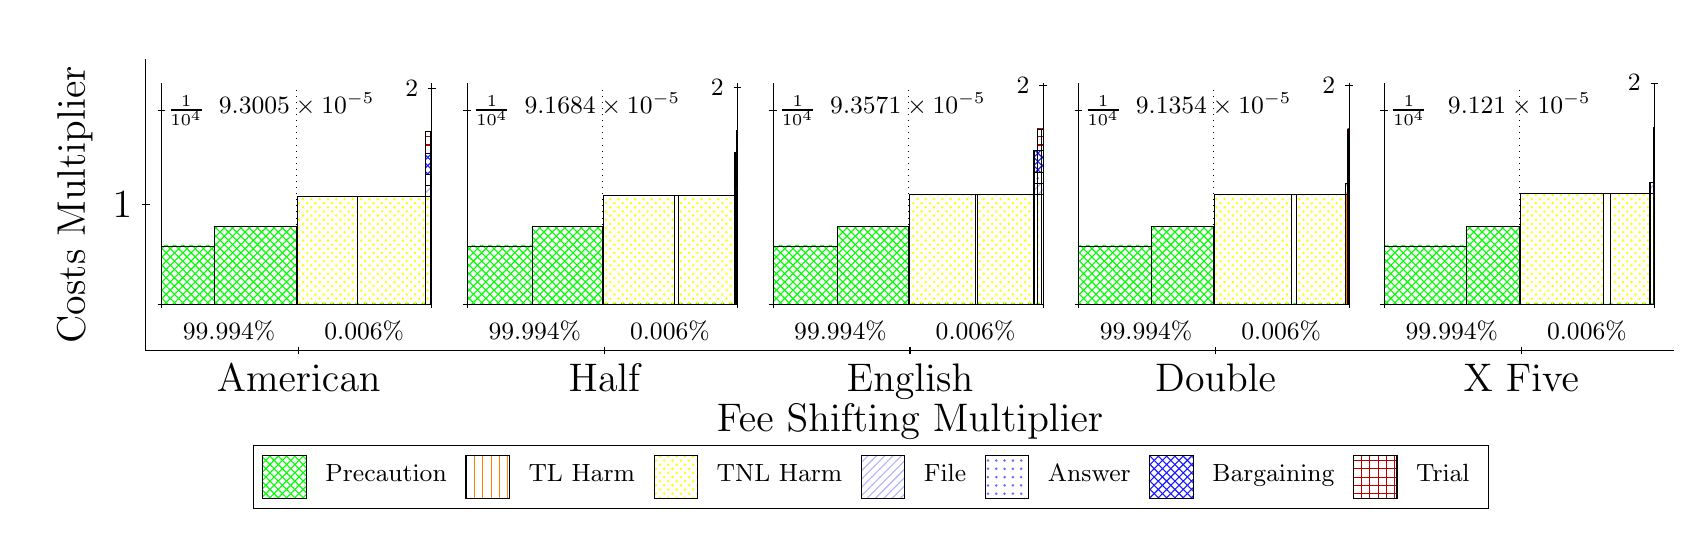
\begin{tikzpicture}
\clip(-0.5,-1.1) rectangle +(20.91,6.2);
\draw[black] (1,1) -- (1,4.7);
\node[rotate=90, fontscale=2, anchor=center] at (0.1, 2.85) {Costs Multiplier};
\draw[black] (0.95,2.85) -- (1.05,2.85);
\node[fontscale=2, anchor=east] at (0.95, 2.85) {1};

\draw[black] (1,1) -- (20.41,1);
\node[fontscale=2, anchor=center] at (10.705, 0.1) {Fee Shifting Multiplier};
\draw[black] (2.941,0.95) -- (2.941,1.05);
\node[fontscale=2, anchor=north] at (2.941, 0.95) {American};
\draw[black] (6.823,0.95) -- (6.823,1.05);
\node[fontscale=2, anchor=north] at (6.823, 0.95) {Half};
\draw[black] (10.705,0.95) -- (10.705,1.05);
\node[fontscale=2, anchor=north] at (10.705, 0.95) {English};
\draw[black] (14.587,0.95) -- (14.587,1.05);
\node[fontscale=2, anchor=north] at (14.587, 0.95) {Double};
\draw[black] (18.469,0.95) -- (18.469,1.05);
\node[fontscale=2, anchor=north] at (18.469, 0.95) {X Five};


\draw[pattern=crosshatch, pattern color=green,draw=black,very thin] (1.2,1.592) rectangle (1.8725,2.3294);
\draw[pattern=crosshatch, pattern color=green,draw=black,very thin] (1.8725,1.592) rectangle (2.916,2.5752);
\draw[pattern=crosshatch, pattern color=green,draw=black,very thin] (2.916,1.592) rectangle (2.9287,1.592);
\draw[pattern=north east lines, pattern color=blue!30,draw=black,very thin] (2.916,1.592) rectangle (2.9287,1.7287);
\draw[pattern=dots,  pattern color=blue!60,draw=black,very thin] (2.916,1.7287) rectangle (2.9287,1.8654);
\draw[pattern=crosshatch,      pattern color=blue!90,draw=black,very thin] (2.916,1.8654) rectangle (2.9287,2.1388);
\draw[pattern=grid,            pattern color=red!70!black,draw=black,very thin] (2.916,2.1388) rectangle (2.9287,2.4121);
\draw[pattern=crosshatch, pattern color=green,draw=black,very thin] (2.9287,1.592) rectangle (3.6818,1.592);
\draw[pattern=crosshatch dots, pattern color=yellow,draw=black,very thin] (2.9287,1.592) rectangle (3.6818,2.9588);
\draw[pattern=crosshatch, pattern color=green,draw=black,very thin] (3.6818,1.592) rectangle (3.6897,1.592);
\draw[pattern=vertical lines, pattern color=orange,draw=black,very thin] (3.6818,1.592) rectangle (3.6897,2.9588);
\draw[pattern=crosshatch, pattern color=green,draw=black,very thin] (3.6897,1.592) rectangle (4.5556,1.5921);
\draw[pattern=crosshatch dots, pattern color=yellow,draw=black,very thin] (3.6897,1.5921) rectangle (4.5556,2.9588);
\draw[pattern=crosshatch, pattern color=green,draw=black,very thin] (4.5556,1.592) rectangle (4.6122,1.592);
\draw[pattern=crosshatch dots, pattern color=yellow,draw=black,very thin] (4.5556,1.592) rectangle (4.6122,2.9588);
\draw[pattern=north east lines, pattern color=blue!30,draw=black,very thin] (4.5556,2.9588) rectangle (4.6122,3.0955);
\draw[pattern=dots,  pattern color=blue!60,draw=black,very thin] (4.5556,3.0955) rectangle (4.6122,3.2322);
\draw[pattern=crosshatch,      pattern color=blue!90,draw=black,very thin] (4.5556,3.2322) rectangle (4.6122,3.5055);
\draw[pattern=grid,            pattern color=red!70!black,draw=black,very thin] (4.5556,3.5055) rectangle (4.6122,3.7789);
\draw[pattern=crosshatch, pattern color=green,draw=black,very thin] (4.6122,1.592) rectangle (4.632,1.592);
\draw[pattern=vertical lines, pattern color=orange,draw=black,very thin] (4.6122,1.592) rectangle (4.632,2.9588);
\draw[pattern=north east lines, pattern color=blue!30,draw=black,very thin] (4.6122,2.9588) rectangle (4.632,3.0955);
\draw[pattern=dots,  pattern color=blue!60,draw=black,very thin] (4.6122,3.0955) rectangle (4.632,3.2322);
\draw[pattern=crosshatch,      pattern color=blue!90,draw=black,very thin] (4.6122,3.2322) rectangle (4.632,3.5055);
\draw[pattern=grid,            pattern color=red!70!black,draw=black,very thin] (4.6122,3.5055) rectangle (4.632,3.7789);
\node[font=\small,text=black,anchor=north] at (2.916, 4.4) {$9.3005\times 10^{-5}$};
\draw[black,very thin] (1.2,1.592) -- (1.2,4.4);
\draw[black,very thin] (1.15,1.592) -- (1.25,1.592);
\node[font=\small,text=black, anchor=west] at (1.15, 1.592) {};
\draw[black,very thin] (1.15,4.0499) -- (1.25,4.0499);
\node[font=\small,text=black, anchor=west] at (1.15, 4.0499) {$\frac{1}{10^{4}}$};

\draw[black,dotted,very thin] (2.916,1.6762) -- (2.916,4.3158);
\draw[black,very thin] (4.632,1.592) -- (4.632,4.4);
\draw[black,very thin] (4.582,4.3256) -- (4.682,4.3256);
\node[font=\small,text=black, anchor=east] at (4.582, 4.3256) {\contour{white}{2}};

\draw[black,very thin] (1.2,1.592) -- (4.632,1.592);
\draw[black,very thin] (1.2,1.542) -- (1.2,1.642);
\node[font=\small,text=black, anchor=north] at (1.2, 1.542) {};
\draw[black,very thin] (4.632,1.542) -- (4.632,1.642);
\node[font=\small,text=black, anchor=north] at (4.632, 1.542) {};

\node[font=\small,text=black,anchor=south] at (2.058, 0.992) {99.994\%};
\node[font=\small,text=black,anchor=south] at (3.774, 0.992) {0.006\%};

\draw[pattern=crosshatch, pattern color=green,draw=black,very thin] (5.082,1.592) rectangle (5.9048,2.3294);
\draw[pattern=crosshatch, pattern color=green,draw=black,very thin] (5.9048,1.592) rectangle (6.798,2.5752);
\draw[pattern=crosshatch, pattern color=green,draw=black,very thin] (6.798,1.592) rectangle (6.8015,1.592);
\draw[pattern=north east lines, pattern color=blue!30,draw=black,very thin] (6.798,1.592) rectangle (6.8015,1.7298);
\draw[pattern=dots,  pattern color=blue!60,draw=black,very thin] (6.798,1.7298) rectangle (6.8015,1.8675);
\draw[pattern=crosshatch,      pattern color=blue!90,draw=black,very thin] (6.798,1.8675) rectangle (6.8015,2.1429);
\draw[pattern=crosshatch, pattern color=green,draw=black,very thin] (6.8015,1.592) rectangle (6.8044,1.592);
\draw[pattern=north east lines, pattern color=blue!30,draw=black,very thin] (6.8015,1.592) rectangle (6.8044,1.7298);
\draw[pattern=dots,  pattern color=blue!60,draw=black,very thin] (6.8015,1.7298) rectangle (6.8044,1.8675);
\draw[pattern=crosshatch,      pattern color=blue!90,draw=black,very thin] (6.8015,1.8675) rectangle (6.8044,2.1429);
\draw[pattern=grid,            pattern color=red!70!black,draw=black,very thin] (6.8015,2.1429) rectangle (6.8044,2.4184);
\draw[pattern=crosshatch, pattern color=green,draw=black,very thin] (6.8044,1.592) rectangle (7.7106,1.592);
\draw[pattern=crosshatch dots, pattern color=yellow,draw=black,very thin] (6.8044,1.592) rectangle (7.7106,2.9692);
\draw[pattern=crosshatch, pattern color=green,draw=black,very thin] (7.7106,1.592) rectangle (7.7626,1.592);
\draw[pattern=vertical lines, pattern color=orange,draw=black,very thin] (7.7106,1.592) rectangle (7.7626,2.9692);
\draw[pattern=crosshatch, pattern color=green,draw=black,very thin] (7.7626,1.592) rectangle (8.4795,1.5921);
\draw[pattern=crosshatch dots, pattern color=yellow,draw=black,very thin] (7.7626,1.5921) rectangle (8.4795,2.9693);
\draw[pattern=crosshatch, pattern color=green,draw=black,very thin] (8.4795,1.592) rectangle (8.4824,1.592);
\draw[pattern=crosshatch dots, pattern color=yellow,draw=black,very thin] (8.4795,1.592) rectangle (8.4824,2.9692);
\draw[pattern=north east lines, pattern color=blue!30,draw=black,very thin] (8.4795,2.9692) rectangle (8.4824,3.107);
\draw[pattern=dots,  pattern color=blue!60,draw=black,very thin] (8.4795,3.107) rectangle (8.4824,3.2447);
\draw[pattern=crosshatch,      pattern color=blue!90,draw=black,very thin] (8.4795,3.2447) rectangle (8.4824,3.5201);
\draw[pattern=crosshatch, pattern color=green,draw=black,very thin] (8.4824,1.592) rectangle (8.4977,1.592);
\draw[pattern=vertical lines, pattern color=orange,draw=black,very thin] (8.4824,1.592) rectangle (8.4977,2.9692);
\draw[pattern=north east lines, pattern color=blue!30,draw=black,very thin] (8.4824,2.9692) rectangle (8.4977,3.107);
\draw[pattern=dots,  pattern color=blue!60,draw=black,very thin] (8.4824,3.107) rectangle (8.4977,3.2447);
\draw[pattern=crosshatch,      pattern color=blue!90,draw=black,very thin] (8.4824,3.2447) rectangle (8.4977,3.5201);
\draw[pattern=crosshatch, pattern color=green,draw=black,very thin] (8.4977,1.592) rectangle (8.5058,1.592);
\draw[pattern=crosshatch dots, pattern color=yellow,draw=black,very thin] (8.4977,1.592) rectangle (8.5058,2.9692);
\draw[pattern=north east lines, pattern color=blue!30,draw=black,very thin] (8.4977,2.9692) rectangle (8.5058,3.107);
\draw[pattern=dots,  pattern color=blue!60,draw=black,very thin] (8.4977,3.107) rectangle (8.5058,3.2447);
\draw[pattern=crosshatch,      pattern color=blue!90,draw=black,very thin] (8.4977,3.2447) rectangle (8.5058,3.5201);
\draw[pattern=grid,            pattern color=red!70!black,draw=black,very thin] (8.4977,3.5201) rectangle (8.5058,3.7956);
\draw[pattern=crosshatch, pattern color=green,draw=black,very thin] (8.5058,1.592) rectangle (8.514,1.592);
\draw[pattern=vertical lines, pattern color=orange,draw=black,very thin] (8.5058,1.592) rectangle (8.514,2.9692);
\draw[pattern=north east lines, pattern color=blue!30,draw=black,very thin] (8.5058,2.9692) rectangle (8.514,3.107);
\draw[pattern=dots,  pattern color=blue!60,draw=black,very thin] (8.5058,3.107) rectangle (8.514,3.2447);
\draw[pattern=crosshatch,      pattern color=blue!90,draw=black,very thin] (8.5058,3.2447) rectangle (8.514,3.5201);
\draw[pattern=grid,            pattern color=red!70!black,draw=black,very thin] (8.5058,3.5201) rectangle (8.514,3.7956);
\node[font=\small,text=black,anchor=north] at (6.798, 4.4) {$9.1684\times 10^{-5}$};
\draw[black,very thin] (5.082,1.592) -- (5.082,4.4);
\draw[black,very thin] (5.032,1.592) -- (5.132,1.592);
\node[font=\small,text=black, anchor=west] at (5.032, 1.592) {};
\draw[black,very thin] (5.032,4.0499) -- (5.132,4.0499);
\node[font=\small,text=black, anchor=west] at (5.032, 4.0499) {$\frac{1}{10^{4}}$};

\draw[black,dotted,very thin] (6.798,1.6762) -- (6.798,4.3158);
\draw[black,very thin] (8.514,1.592) -- (8.514,4.4);
\draw[black,very thin] (8.464,4.3464) -- (8.564,4.3464);
\node[font=\small,text=black, anchor=east] at (8.464, 4.3464) {\contour{white}{2}};

\draw[black,very thin] (5.082,1.592) -- (8.514,1.592);
\draw[black,very thin] (5.082,1.542) -- (5.082,1.642);
\node[font=\small,text=black, anchor=north] at (5.082, 1.542) {};
\draw[black,very thin] (8.514,1.542) -- (8.514,1.642);
\node[font=\small,text=black, anchor=north] at (8.514, 1.542) {};

\node[font=\small,text=black,anchor=south] at (5.94, 0.992) {99.994\%};
\node[font=\small,text=black,anchor=south] at (7.656, 0.992) {0.006\%};

\draw[pattern=crosshatch, pattern color=green,draw=black,very thin] (8.964,1.592) rectangle (9.7862,2.3294);
\draw[pattern=crosshatch, pattern color=green,draw=black,very thin] (9.7862,1.592) rectangle (10.68,2.5752);
\draw[pattern=crosshatch, pattern color=green,draw=black,very thin] (10.68,1.592) rectangle (10.69,1.592);
\draw[pattern=north east lines, pattern color=blue!30,draw=black,very thin] (10.68,1.592) rectangle (10.69,1.731);
\draw[pattern=dots,  pattern color=blue!60,draw=black,very thin] (10.68,1.731) rectangle (10.69,1.87);
\draw[pattern=crosshatch,      pattern color=blue!90,draw=black,very thin] (10.68,1.87) rectangle (10.69,2.148);
\draw[pattern=crosshatch, pattern color=green,draw=black,very thin] (10.69,1.592) rectangle (10.702,1.592);
\draw[pattern=north east lines, pattern color=blue!30,draw=black,very thin] (10.69,1.592) rectangle (10.702,1.731);
\draw[pattern=dots,  pattern color=blue!60,draw=black,very thin] (10.69,1.731) rectangle (10.702,1.87);
\draw[pattern=crosshatch,      pattern color=blue!90,draw=black,very thin] (10.69,1.87) rectangle (10.702,2.148);
\draw[pattern=grid,            pattern color=red!70!black,draw=black,very thin] (10.69,2.148) rectangle (10.702,2.426);
\draw[pattern=crosshatch, pattern color=green,draw=black,very thin] (10.702,1.592) rectangle (11.537,1.592);
\draw[pattern=crosshatch dots, pattern color=yellow,draw=black,very thin] (10.702,1.592) rectangle (11.537,2.9819);
\draw[pattern=crosshatch, pattern color=green,draw=black,very thin] (11.537,1.592) rectangle (11.558,1.592);
\draw[pattern=vertical lines, pattern color=orange,draw=black,very thin] (11.537,1.592) rectangle (11.558,2.9819);
\draw[pattern=crosshatch, pattern color=green,draw=black,very thin] (11.558,1.592) rectangle (12.269,1.5921);
\draw[pattern=crosshatch dots, pattern color=yellow,draw=black,very thin] (11.558,1.5921) rectangle (12.269,2.9819);
\draw[pattern=crosshatch, pattern color=green,draw=black,very thin] (12.269,1.592) rectangle (12.287,1.592);
\draw[pattern=crosshatch dots, pattern color=yellow,draw=black,very thin] (12.269,1.592) rectangle (12.287,2.9819);
\draw[pattern=north east lines, pattern color=blue!30,draw=black,very thin] (12.269,2.9819) rectangle (12.287,3.1209);
\draw[pattern=dots,  pattern color=blue!60,draw=black,very thin] (12.269,3.1209) rectangle (12.287,3.2599);
\draw[pattern=crosshatch,      pattern color=blue!90,draw=black,very thin] (12.269,3.2599) rectangle (12.287,3.5379);
\draw[pattern=crosshatch, pattern color=green,draw=black,very thin] (12.287,1.592) rectangle (12.321,1.592);
\draw[pattern=vertical lines, pattern color=orange,draw=black,very thin] (12.287,1.592) rectangle (12.321,2.9819);
\draw[pattern=north east lines, pattern color=blue!30,draw=black,very thin] (12.287,2.9819) rectangle (12.321,3.1209);
\draw[pattern=dots,  pattern color=blue!60,draw=black,very thin] (12.287,3.1209) rectangle (12.321,3.2599);
\draw[pattern=crosshatch,      pattern color=blue!90,draw=black,very thin] (12.287,3.2599) rectangle (12.321,3.5379);
\draw[pattern=crosshatch, pattern color=green,draw=black,very thin] (12.321,1.592) rectangle (12.377,1.592);
\draw[pattern=crosshatch dots, pattern color=yellow,draw=black,very thin] (12.321,1.592) rectangle (12.377,2.9819);
\draw[pattern=north east lines, pattern color=blue!30,draw=black,very thin] (12.321,2.9819) rectangle (12.377,3.1209);
\draw[pattern=dots,  pattern color=blue!60,draw=black,very thin] (12.321,3.1209) rectangle (12.377,3.2599);
\draw[pattern=crosshatch,      pattern color=blue!90,draw=black,very thin] (12.321,3.2599) rectangle (12.377,3.5379);
\draw[pattern=grid,            pattern color=red!70!black,draw=black,very thin] (12.321,3.5379) rectangle (12.377,3.8158);
\draw[pattern=crosshatch, pattern color=green,draw=black,very thin] (12.377,1.592) rectangle (12.396,1.592);
\draw[pattern=vertical lines, pattern color=orange,draw=black,very thin] (12.377,1.592) rectangle (12.396,2.9819);
\draw[pattern=north east lines, pattern color=blue!30,draw=black,very thin] (12.377,2.9819) rectangle (12.396,3.1209);
\draw[pattern=dots,  pattern color=blue!60,draw=black,very thin] (12.377,3.1209) rectangle (12.396,3.2599);
\draw[pattern=crosshatch,      pattern color=blue!90,draw=black,very thin] (12.377,3.2599) rectangle (12.396,3.5379);
\draw[pattern=grid,            pattern color=red!70!black,draw=black,very thin] (12.377,3.5379) rectangle (12.396,3.8158);
\node[font=\small,text=black,anchor=north] at (10.68, 4.4) {$9.3571\times 10^{-5}$};
\draw[black,very thin] (8.964,1.592) -- (8.964,4.4);
\draw[black,very thin] (8.914,1.592) -- (9.014,1.592);
\node[font=\small,text=black, anchor=west] at (8.914, 1.592) {};
\draw[black,very thin] (8.914,4.0499) -- (9.014,4.0499);
\node[font=\small,text=black, anchor=west] at (8.914, 4.0499) {$\frac{1}{10^{4}}$};

\draw[black,dotted,very thin] (10.68,1.6762) -- (10.68,4.3158);
\draw[black,very thin] (12.396,1.592) -- (12.396,4.4);
\draw[black,very thin] (12.346,4.3717) -- (12.446,4.3717);
\node[font=\small,text=black, anchor=east] at (12.346, 4.3717) {\contour{white}{2}};

\draw[black,very thin] (8.964,1.592) -- (12.396,1.592);
\draw[black,very thin] (8.964,1.542) -- (8.964,1.642);
\node[font=\small,text=black, anchor=north] at (8.964, 1.542) {};
\draw[black,very thin] (12.396,1.542) -- (12.396,1.642);
\node[font=\small,text=black, anchor=north] at (12.396, 1.542) {};

\node[font=\small,text=black,anchor=south] at (9.822, 0.992) {99.994\%};
\node[font=\small,text=black,anchor=south] at (11.538, 0.992) {0.006\%};

\draw[pattern=crosshatch, pattern color=green,draw=black,very thin] (12.846,1.592) rectangle (13.769,2.3294);
\draw[pattern=crosshatch, pattern color=green,draw=black,very thin] (13.769,1.592) rectangle (14.562,2.5752);
\draw[pattern=crosshatch, pattern color=green,draw=black,very thin] (14.562,1.592) rectangle (14.568,1.592);
\draw[pattern=north east lines, pattern color=blue!30,draw=black,very thin] (14.562,1.592) rectangle (14.568,1.731);
\draw[pattern=crosshatch, pattern color=green,draw=black,very thin] (14.568,1.592) rectangle (14.571,1.592);
\draw[pattern=north east lines, pattern color=blue!30,draw=black,very thin] (14.568,1.592) rectangle (14.571,1.731);
\draw[pattern=dots,  pattern color=blue!60,draw=black,very thin] (14.568,1.731) rectangle (14.571,1.8699);
\draw[pattern=crosshatch,      pattern color=blue!90,draw=black,very thin] (14.568,1.8699) rectangle (14.571,2.1478);
\draw[pattern=grid,            pattern color=red!70!black,draw=black,very thin] (14.568,2.1478) rectangle (14.571,2.4257);
\draw[pattern=crosshatch, pattern color=green,draw=black,very thin] (14.571,1.592) rectangle (15.542,1.592);
\draw[pattern=crosshatch dots, pattern color=yellow,draw=black,very thin] (14.571,1.592) rectangle (15.542,2.9814);
\draw[pattern=crosshatch, pattern color=green,draw=black,very thin] (15.542,1.592) rectangle (15.615,1.592);
\draw[pattern=vertical lines, pattern color=orange,draw=black,very thin] (15.542,1.592) rectangle (15.615,2.9814);
\draw[pattern=crosshatch, pattern color=green,draw=black,very thin] (15.615,1.592) rectangle (16.232,1.5921);
\draw[pattern=crosshatch dots, pattern color=yellow,draw=black,very thin] (15.615,1.5921) rectangle (16.232,2.9815);
\draw[pattern=crosshatch, pattern color=green,draw=black,very thin] (16.232,1.592) rectangle (16.237,1.592);
\draw[pattern=crosshatch dots, pattern color=yellow,draw=black,very thin] (16.232,1.592) rectangle (16.237,2.9814);
\draw[pattern=north east lines, pattern color=blue!30,draw=black,very thin] (16.232,2.9814) rectangle (16.237,3.1204);
\draw[pattern=crosshatch, pattern color=green,draw=black,very thin] (16.237,1.592) rectangle (16.262,1.592);
\draw[pattern=vertical lines, pattern color=orange,draw=black,very thin] (16.237,1.592) rectangle (16.262,2.9814);
\draw[pattern=north east lines, pattern color=blue!30,draw=black,very thin] (16.237,2.9814) rectangle (16.262,3.1204);
\draw[pattern=crosshatch, pattern color=green,draw=black,very thin] (16.262,1.592) rectangle (16.27,1.592);
\draw[pattern=crosshatch dots, pattern color=yellow,draw=black,very thin] (16.262,1.592) rectangle (16.27,2.9814);
\draw[pattern=north east lines, pattern color=blue!30,draw=black,very thin] (16.262,2.9814) rectangle (16.27,3.1204);
\draw[pattern=dots,  pattern color=blue!60,draw=black,very thin] (16.262,3.1204) rectangle (16.27,3.2593);
\draw[pattern=crosshatch,      pattern color=blue!90,draw=black,very thin] (16.262,3.2593) rectangle (16.27,3.5372);
\draw[pattern=grid,            pattern color=red!70!black,draw=black,very thin] (16.262,3.5372) rectangle (16.27,3.8151);
\draw[pattern=crosshatch, pattern color=green,draw=black,very thin] (16.27,1.592) rectangle (16.278,1.592);
\draw[pattern=vertical lines, pattern color=orange,draw=black,very thin] (16.27,1.592) rectangle (16.278,2.9814);
\draw[pattern=north east lines, pattern color=blue!30,draw=black,very thin] (16.27,2.9814) rectangle (16.278,3.1204);
\draw[pattern=dots,  pattern color=blue!60,draw=black,very thin] (16.27,3.1204) rectangle (16.278,3.2593);
\draw[pattern=crosshatch,      pattern color=blue!90,draw=black,very thin] (16.27,3.2593) rectangle (16.278,3.5372);
\draw[pattern=grid,            pattern color=red!70!black,draw=black,very thin] (16.27,3.5372) rectangle (16.278,3.8151);
\node[font=\small,text=black,anchor=north] at (14.562, 4.4) {$9.1354\times 10^{-5}$};
\draw[black,very thin] (12.846,1.592) -- (12.846,4.4);
\draw[black,very thin] (12.796,1.592) -- (12.896,1.592);
\node[font=\small,text=black, anchor=west] at (12.796, 1.592) {};
\draw[black,very thin] (12.796,4.0499) -- (12.896,4.0499);
\node[font=\small,text=black, anchor=west] at (12.796, 4.0499) {$\frac{1}{10^{4}}$};

\draw[black,dotted,very thin] (14.562,1.6762) -- (14.562,4.3158);
\draw[black,very thin] (16.278,1.592) -- (16.278,4.4);
\draw[black,very thin] (16.228,4.3708) -- (16.328,4.3708);
\node[font=\small,text=black, anchor=east] at (16.228, 4.3708) {\contour{white}{2}};

\draw[black,very thin] (12.846,1.592) -- (16.278,1.592);
\draw[black,very thin] (12.846,1.542) -- (12.846,1.642);
\node[font=\small,text=black, anchor=north] at (12.846, 1.542) {};
\draw[black,very thin] (16.278,1.542) -- (16.278,1.642);
\node[font=\small,text=black, anchor=north] at (16.278, 1.542) {};

\node[font=\small,text=black,anchor=south] at (13.704, 0.992) {99.994\%};
\node[font=\small,text=black,anchor=south] at (15.42, 0.992) {0.006\%};

\draw[pattern=crosshatch, pattern color=green,draw=black,very thin] (16.728,1.592) rectangle (17.772,2.3294);
\draw[pattern=crosshatch, pattern color=green,draw=black,very thin] (17.772,1.592) rectangle (18.444,2.5752);
\draw[pattern=crosshatch, pattern color=green,draw=black,very thin] (18.444,1.592) rectangle (18.452,1.592);
\draw[pattern=north east lines, pattern color=blue!30,draw=black,very thin] (18.444,1.592) rectangle (18.452,1.7324);
\draw[pattern=crosshatch, pattern color=green,draw=black,very thin] (18.452,1.592) rectangle (18.455,1.592);
\draw[pattern=north east lines, pattern color=blue!30,draw=black,very thin] (18.452,1.592) rectangle (18.455,1.7324);
\draw[pattern=dots,  pattern color=blue!60,draw=black,very thin] (18.452,1.7324) rectangle (18.455,1.8728);
\draw[pattern=crosshatch,      pattern color=blue!90,draw=black,very thin] (18.452,1.8728) rectangle (18.455,2.1536);
\draw[pattern=grid,            pattern color=red!70!black,draw=black,very thin] (18.452,2.1536) rectangle (18.455,2.4344);
\draw[pattern=crosshatch, pattern color=green,draw=black,very thin] (18.455,1.592) rectangle (19.504,1.592);
\draw[pattern=crosshatch dots, pattern color=yellow,draw=black,very thin] (18.455,1.592) rectangle (19.504,2.996);
\draw[pattern=crosshatch, pattern color=green,draw=black,very thin] (19.504,1.592) rectangle (19.602,1.592);
\draw[pattern=vertical lines, pattern color=orange,draw=black,very thin] (19.504,1.592) rectangle (19.602,2.996);
\draw[pattern=crosshatch, pattern color=green,draw=black,very thin] (19.602,1.592) rectangle (20.1,1.5921);
\draw[pattern=crosshatch dots, pattern color=yellow,draw=black,very thin] (19.602,1.5921) rectangle (20.1,2.996);
\draw[pattern=crosshatch, pattern color=green,draw=black,very thin] (20.1,1.592) rectangle (20.107,1.592);
\draw[pattern=crosshatch dots, pattern color=yellow,draw=black,very thin] (20.1,1.592) rectangle (20.107,2.996);
\draw[pattern=north east lines, pattern color=blue!30,draw=black,very thin] (20.1,2.996) rectangle (20.107,3.1364);
\draw[pattern=crosshatch, pattern color=green,draw=black,very thin] (20.107,1.592) rectangle (20.144,1.592);
\draw[pattern=vertical lines, pattern color=orange,draw=black,very thin] (20.107,1.592) rectangle (20.144,2.996);
\draw[pattern=north east lines, pattern color=blue!30,draw=black,very thin] (20.107,2.996) rectangle (20.144,3.1364);
\draw[pattern=crosshatch, pattern color=green,draw=black,very thin] (20.144,1.592) rectangle (20.152,1.592);
\draw[pattern=crosshatch dots, pattern color=yellow,draw=black,very thin] (20.144,1.592) rectangle (20.152,2.996);
\draw[pattern=north east lines, pattern color=blue!30,draw=black,very thin] (20.144,2.996) rectangle (20.152,3.1364);
\draw[pattern=dots,  pattern color=blue!60,draw=black,very thin] (20.144,3.1364) rectangle (20.152,3.2768);
\draw[pattern=crosshatch,      pattern color=blue!90,draw=black,very thin] (20.144,3.2768) rectangle (20.152,3.5576);
\draw[pattern=grid,            pattern color=red!70!black,draw=black,very thin] (20.144,3.5576) rectangle (20.152,3.8384);
\draw[pattern=crosshatch, pattern color=green,draw=black,very thin] (20.152,1.592) rectangle (20.16,1.592);
\draw[pattern=vertical lines, pattern color=orange,draw=black,very thin] (20.152,1.592) rectangle (20.16,2.996);
\draw[pattern=north east lines, pattern color=blue!30,draw=black,very thin] (20.152,2.996) rectangle (20.16,3.1364);
\draw[pattern=dots,  pattern color=blue!60,draw=black,very thin] (20.152,3.1364) rectangle (20.16,3.2768);
\draw[pattern=crosshatch,      pattern color=blue!90,draw=black,very thin] (20.152,3.2768) rectangle (20.16,3.5576);
\draw[pattern=grid,            pattern color=red!70!black,draw=black,very thin] (20.152,3.5576) rectangle (20.16,3.8384);
\node[font=\small,text=black,anchor=north] at (18.444, 4.4) {$9.121\times 10^{-5}$};
\draw[black,very thin] (16.728,1.592) -- (16.728,4.4);
\draw[black,very thin] (16.678,1.592) -- (16.778,1.592);
\node[font=\small,text=black, anchor=west] at (16.678, 1.592) {};
\draw[black,very thin] (16.678,4.0499) -- (16.778,4.0499);
\node[font=\small,text=black, anchor=west] at (16.678, 4.0499) {$\frac{1}{10^{4}}$};

\draw[black,dotted,very thin] (18.444,1.6762) -- (18.444,4.3158);
\draw[black,very thin] (20.16,1.592) -- (20.16,4.4);
\draw[black,very thin] (20.11,4.3999) -- (20.21,4.3999);
\node[font=\small,text=black, anchor=east] at (20.11, 4.3999) {\contour{white}{2}};

\draw[black,very thin] (16.728,1.592) -- (20.16,1.592);
\draw[black,very thin] (16.728,1.542) -- (16.728,1.642);
\node[font=\small,text=black, anchor=north] at (16.728, 1.542) {};
\draw[black,very thin] (20.16,1.542) -- (20.16,1.642);
\node[font=\small,text=black, anchor=north] at (20.16, 1.542) {};

\node[font=\small,text=black,anchor=south] at (17.586, 0.992) {99.994\%};
\node[font=\small,text=black,anchor=south] at (19.302, 0.992) {0.006\%};

\coordinate (LegendAnchor) at (10.205000000000002,0);
\begin{scope}[align=center]
\matrix[scale=0.6,draw=black,below=0.2cm of LegendAnchor,nodes={draw},column sep=0.12cm]{
\node[rectangle,draw,minimum width=0.55cm,minimum height=0.55cm,pattern=crosshatch, pattern color=green]{}; &
        \node[draw=none,font=\small]{Precaution}; &
\node[rectangle,draw,minimum width=0.55cm,minimum height=0.55cm,pattern=vertical lines, pattern color=orange]{}; &
        \node[draw=none,font=\small]{TL Harm}; &
\node[rectangle,draw,minimum width=0.55cm,minimum height=0.55cm,pattern=crosshatch dots, pattern color=yellow]{}; &
        \node[draw=none,font=\small]{TNL Harm}; &
\node[rectangle,draw,minimum width=0.55cm,minimum height=0.55cm,pattern=north east lines, pattern color=blue!30]{}; &
        \node[draw=none,font=\small]{File}; &
\node[rectangle,draw,minimum width=0.55cm,minimum height=0.55cm,pattern=dots, pattern color=blue!60]{}; &
        \node[draw=none,font=\small]{Answer}; &
\node[rectangle,draw,minimum width=0.55cm,minimum height=0.55cm,pattern=crosshatch, pattern color=blue!90]{}; &
        \node[draw=none,font=\small]{Bargaining}; &
\node[rectangle,draw,minimum width=0.55cm,minimum height=0.55cm,pattern=grid, pattern color=red!70!black]{}; &
        \node[draw=none,font=\small]{Trial}; \\
};\end{scope}

\end{tikzpicture}
\end{document}